
\textbf{Detailed Analysis}

Figure \ref{fig:atari_results} demonstrates that both positive and
negative transfer is possible with progressive nets. To differentiate
these cases, we consider the Average Fisher Sensitivity for the 3 column
case (e.g., see Fig.~\ref{fig:atari3_results_neil}a). A clear pattern
emerges amongst these and other examples: the most negative transfer
coincides with complete dependence on the convolutional layers of the
previous columns, and no learning of new visual features in the new
column. In contrast, the most positive transfer occurs when the
features of the first two columns are \textit{augmented} by
new features. The statistics across all 3-column nets
(Figure \ref{fig:atari3_results_neil}b) show that positive transfer in
Atari occurs at a "sweet spot" between heavy reliance on features from
the source task, and heavy reliance on all new features for the
target task.

\begin{figure}[h]
  \centering 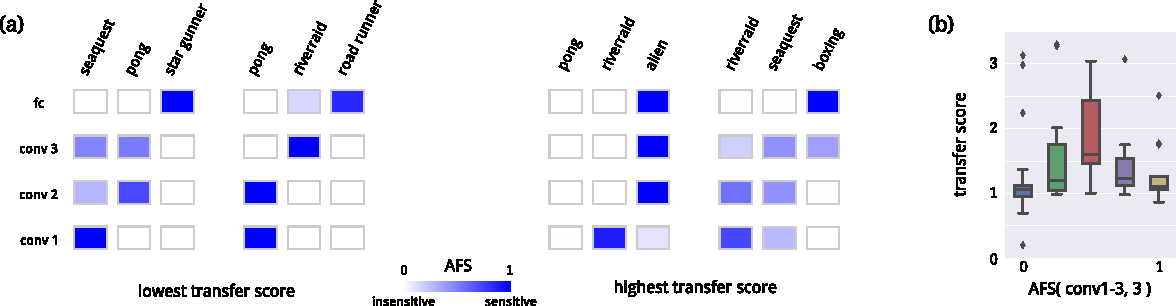
\includegraphics[width=.95\textwidth]{figures/atari3_results_neil.pdf} \caption{(a)
    AFS scores for 3-column nets with lowest (left) and highest
    (right) transfer scores on the 12 target Atari games. (b) Transfer
    statistics across 72 three-column nets, as a function of the
    mean AFS across the three convolutional layers of the new
    column (i.e.\ how much new vision is learned). } \label{fig:atari3_results_neil}
\end{figure}

At first glance, this result appears unintuitive: if a progressive net
finds a valuable feature set from a source task,
shouldn't we expect a high degree of transfer?
We offer two hypotheses. First, this may
simply reflect an optimization difficulty, where the source features offer
fast convergence to a poor local minimum. This is a known
challenge in transfer learning \cite{AAAIMag11-Taylor}: learned source
tasks confer an inductive bias that can either help or hinder in different cases.
Second, this may reflect a problem of
exploration, where the transfered representation is "good enough" for
a functional, but sub-optimal policy. 





